
\documentclass[12pt]{article}
\usepackage{helvet}
\renewcommand{\familydefault}{\sfdefault}
\usepackage{hyperref}
\usepackage[english]{babel}
\usepackage[utf8]{inputenc}
\usepackage{amsmath}
\usepackage{graphicx}
\usepackage{cite}
\usepackage{xspace}
\usepackage{algorithmicx}
\usepackage[noend]{algpseudocode}
\usepackage{algorithm}
\usepackage[colorinlistoftodos]{todonotes}
\usepackage{setspace}
\onehalfspacing

%\usepackage[notablist,nofiglist]{endfloat}

% Add Yield as a pseudocode command
\algnewcommand\algorithmicyield{\textbf{yield}}
\algnewcommand\Yield{\algorithmicyield{} }%

% Add Continue as a pseudocode command
\algnewcommand\algorithmiccontinue{\textbf{continue}}
\algnewcommand\Continue{\algorithmiccontinue{} }%

% Add Break as a pseudocode command
\algnewcommand\algorithmicbreak{\textbf{break}}
\algnewcommand\Break{\algorithmicbreak{} }%

% Non-useless comments
\algrenewcomment[1]{\(\triangleright\) #1}%

% Have a command for vocab words
\newcommand{\vocab}[1]{\textbf{#1}\xspace}

\newcommand{\vg}{{\tt vg}}
\newcommand{\gcsa}{{\tt GCSA2}}

\begin{document}

\title{Sequence variation aware references and read mapping with vg: the variation graph toolkit}

\author{Erik Garrison 1, Adam Novak 2, Glenn Hickey 2, Jouni Siren 1, Eric
  Dawson 1, Will Jones 1, Orion Buske 3, Mike Lin 4, Benedict Paten 2,
  Richard Durbin 1}

\maketitle

\begin{abstract}
Reference genomes provide a prior to guide our interpretation of DNA sequence data.
However, standard linear reference sequences have a fundamental limitation in that they only represent one version of each locus, whereas
in a population or species there is in general a distribution of related sequences at each locus.
Mapping sequence read data from new individuals to a single linear reference can introduce bias and other problems.
\emph{Variation graphs}, which are bidirectional DNA sequence graphs that capture , describe general sequences of interest as walks through the graph.
Here we enable the practical use of variation graphs at human genome scale, allow the representation of alternate genomes in the reference system.
by building a toolkit of computational methods for the creation, manipulation, and utilization of these structures.
Using generalised compressed suffix array technology we provide an efficient approach to mapping reads onto our graphs.
Our approach generalizes fundamental aspects of resequencing analysis (assembly, alignment, variant calling, and genotyping) to operate on variation graphs.
\end{abstract}

\section{Introduction}

Where genomes are small and sequences from different individuals can be reliably isolated, we can understand variation by assembling whole genomes and then comparing them via whole-genome comparison approaches \cite{mummer}.
In practice, complete de novo genome assemblies are not obtainable for large genomes such as \emph{Homo sapiens}, and we require prior information to interpret new sequence data in its correct genomic context.  
The current paradigm is to align sequence reads to a single high quality reference genome sequence obtained from one (or a few)  closely-related individuals.  
While expedient, this approach biases our results towards a reference that may poorly represent alleles present in the sample we obtained our sequence reads from.  
There is even likely to be sequence in the new sample that is not present in the reference {cite BGI pangenome paper}.  

In principle we would like to align to a genome that is as similar to our sample as possible, ideally a ``personalized'' reference genome \cite{Yuan_2012}, which already incorporates sequence variants present in the individual.  
Of course there is a chicken and egg problem in knowing what the variants are before aligning data from a sample, but most differences between any one genome and the reference are shared in the population, so if we can build a structure that contains known shared variation then that could potentially contain most of the correct personalised reference sequence for any individual from the population or species.
The natural computational structure for doing this is the sequence graph.
These have a long history of application to problems which require the representation of multiple genomes or ambiguities in the same structure.
For example, multiple sequence alignments have a natural representation as partially ordered sequence graphs \cite{lee2002POA}.
The variant call format (VCF) \cite{danecek2011}, which is a common data format for describing populations of genomes, does not explicitly define a graph model, but can be understood as defining a partially ordered graph similar to those used in multiple sequence alignment. 
The total information available in a shotgun sequencing data set set can be compressed into a string graph, in which single-copy sequences are represented uniquely and repeated sequences unresolvable due to read lengths are collapsed into single entities \cite{myers2005, simpson2010}.
A similar structure which has good scaling properties when applied to the problem of genome assembly is the de Bruijn graph, which records the relationships between unique $k$-mers of a set of sequences with edges that link pairs of $k$-mers for which the suffix of one $k$-mer is the prefix of the next \cite{iqbal2012}.

To serve as a population variation aware reference system, we adopt a general sequence graph structure. 
A similar approach has been introduced before for localised genomic regions \cite{prg2015}, but here we extend to a wider range of variation, and provide an implementation in a practical software environment for operating with them at the multi-gigabase scale: \vg. 
We demonstrate the use of \vg by constructing a whole human genome graph incorporating all base-pair specific variation from the 1000 Genomes Project \cite{1000g2015} aligning short read sequencing data against it, and reporting genotypes.

\section{Methods}

\subsection{Model}

We define a variation graph to be a graph with embedded paths $G = ( N, E, P )$ comprised of
a set of nodes $N = n_1 \ldots n_M$,
a set of directed edges $E = e_1 \ldots e_L$,
and a set of paths $P = p_1 \ldots p_Q$ which describe embedding of a set of sequences into the graph.

Each node $n_i$ represents a sequence $seq(n_i)$ which is built from an arbitrary alphabet ${ \cal A }$.
For DNA sequences, we use ${ \cal A } = \{ {\tt A, T, G, C, N} \}$, but in principle the model can be based in any alphabet.
Nodes may be traversed in either the forward ($+$) or reverse direction ($-$), with the sequence being reverse-complemented in the
$-$ direction.  
We write $\overline{n_i}$ for the reverse-complement of node $n_i$, so that $seq(n_i) = revcomp(seq(\overline{n_i}))$, and note
that $\overline{\overline{n}} = n$.  Below, where we refer to {\em node} in most places we mean an oriented node. 

Edges represent links between nodes that can be followed in paths to represent longer sequences.
Edges can be identified with the ordered pairs of (oriented) nodes that they link, so we can write
$e_{i \rightarrow j} = ( n_i, n_j ) $.  In fact this defines one strand of an edge.  Edges also can be traversed in either forward or
reverse direction, with the reverse strand defined by $\overline{e_{i \rightarrow j}} = (  \overline{n_j}, \overline{n_i} )$.

We define paths as alignments to a walk through the graph.  Explicitly, a path is a series of {\em mapping} operations, each
describing the segment of the path derived from a single node, $p = m_1, \ldots, m_{|p|}$.  Each mapping $m$ can be written
as $( (n, o), e_i \ldots e_{|m|} )$, where $n$ is the node, $o$ is the zero-offset start position in the node sequence ($0 \le o < |n|$),
and each $e_i$ is an ``edit'' which copies or replaces a segment of the node sequence.  In \vg we encode $e$ as $(f, t, s)$
where $f$ is a length in the node (``from length''), $t$ is a length in the derived sequence (``to length''), and $s$ is an optional
replacement literal sequence of length $t$.  Edges traversed in a path are implicitly defined by the nodes of neighbouring mappings.
If all the edits are copies then we say that the path is {\em fully embedded} in the graph.

Figure \ref{fig:minimhc} provides a visual explanation of this model using a small fragment of an assembly of MHC haplotypes.

\begin{figure}[t]
\centering
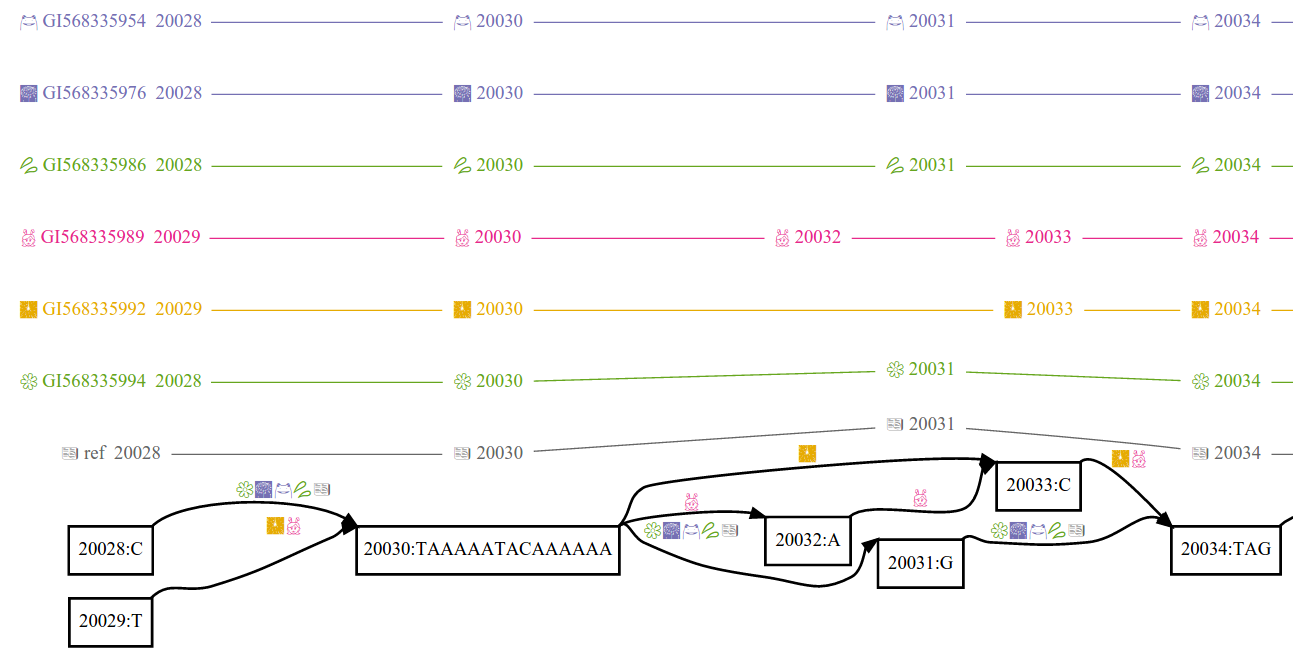
\includegraphics[width=1.0\textwidth]{figures/minimhc}
\caption{\label{fig:minimhc}
  A visualization of a fragment of the MHC variation graph.
  The graph nodes and edges are written at bottom. The edges flow across the tops of the nodes, which indicates in this visualization that they are on the forward strand of the graph and not inverting.
  Paths are described in a matrix above the graph.
  The path name (shown at left) is hashed into a space of 8 colors and 766 Unicode characters (emoji) to provide stable and non-overlapping visual motifs for hundreds of paths.
  These colored pictographs are used to annotate parts of the graph, in this case the edges are labeled with the paths that cross them.
  Visualizations of this type are produced using {\tt vg view -dpn}.
}
\end{figure}

\subsection{Construction}

We can build a trivial graph with a single node and no edges from a linear reference sequence.
A more interesting graph may be generated by a series of align and edit operations.
We first describe our approach to alignment and editing, then summarise a number of interfaces to construct variation graphs using these operations from different types of input information.

\subsubsection{Alignment}

\emph{Alignment} is the process of finding an optimal path to the graph for a new DNA sequence such as a sequencing read.
Our approach to this is to find seed matches by an indexed search process, cluster them if there are multiple nearby seeds, and then perform local dynamic programming alignment of the read into a region of the graph around the seeds.  
We discuss how we find seeds below in \ref{sec:GCSA2}.
When it comes to local dynamic programming, we must deal with the issue that \vg supports arbitrary sequence graphs, which may contain cycles representing repeats and inversions.  
To avoid the complications introduced by cycles \cite{myers1989}, we transform the local graph region into a directed acyclic graph (DAG), on which we can perform
partial order alignment (POA) \cite{lee2002POA}, which generalizes standard pairwise sequence alignment by considering all possible inbound 
positions in the graph in the recursion that derives the score for a new cell.

To transform the local graph into a DAG, we introduce {\tt VG::unfold} and {\tt VG::dagify}.  
Unfold duplicates sections of the graph to materialise both the reverse-complement as well as the forward strand of nodes where this is necessary.  
Dagify unrolls loops.  
Both take a length parameter $k$ with the goal that all sequences up to length $k$ are represented in the resulting graph without cycles.
We keep track of the mappings through both these processes, so that we are able to translate alignments to the transformed graph back into the original one.
Further details are given in the Appendix.

To carry out the partial order alignment, we extended a SIMD-accelerated implementation \cite{zhao2013} of Farrar's  striped Smith Waterman (SSW) algorithm \cite{farrar2007}, which we term ``graph striped Smith-Waterman'' \href{https://github.com/ekg/gssw}{GSSW}.
GSSW generalizes all aspects of SSW to operate over sequence DAGs, including affine gap penalties, retains its matrices for traceback, and is around six times faster than a non-SIMD based implementation of POA.

\subsubsection{Editing}

The operation $edit(G, P)$ extends the graph $G$ to include the sequences described by paths $P$, so that they become fully embedded.

If the nodes of the graph have single-base labels, then they are atomic and we only need to add edges and new nodes representing novel sequence.
We walk the mappings of the path through the graph.
We make no changes for matches.
For substitutions, and insertions, we add the novel sequence from the path edit as new single base nodes in the graph.
For deletions we add edges between existing nodes in the graph.
To edit a non-atomic graph, where the node labels may be of arbitrary length, we first cut nodes in the paths where we need to add new sequence or edges. 

We implement this editing method as \href{https://github.com/vgteam/vg/blob/fbcb6e62/src/vg.cpp#L4846-L4912}{{\tt VG::edit}}, which consumes a set of paths (possibly from alignments) and extends the graph.

\subsubsection{Progressive variation graph construction}

Given a set of alternate genome sequences or fragments of genomes, we can align each sequence in turn and edit the graph to include it.
The resulting graph contains all input sequences as embedded paths.
We implement this technique as the \href{https://github.com/vgteam/vg/blob/fbcb6e62/src/main.cpp#L674-L1248}{multiple sequence/graph aligner {\tt vg msga}}, and have applied it to assemble long sequences from the human MHC as described in section \ref{sec:MHC}.

\subsubsection{Construction from existing population variation data}

Population sequencing projects that have inferred variation from alignments to a linear reference sequence, such as the 1000 Genomes Project, typically generate a file of variants in VCF format.
First, we convert the variants in the VCF file into mappings to a graph made of only the reference sequence. 
We then edit this graph using the mappings, incorporating the sequences given by the alleles in the VCF record into the graph. 
We use this approach below in results section \ref{sec:1000g}.

\subsubsection{Construction from a \emph{de novo} assembly}

Almost all \emph{de novo} assembly algorithms build a sequence graph internally to represent ambiguity in the ways to connect together sequence reads.
They assemble a graph by overlapping reads or their $k$-mers, then generate contigs as non-branching regions of this graph after removing likely sequencing errors.
Provided that an assembler implements export of its graph structure, we can build a variation graph from this intermediate representation.
In \vg we support the \href{https://github.com/pmelsted/GFA-spec}{graphical fragment assembly (GFA) format}, which is a community standard for serialization of bidirectional sequence graphs from assemblers.  There are some complexities in transitioning from an overlap graph formalism to the blunt-end-join model used in \vg, described further in the appendix.

\subsection{Compressed representation and indexing}

Our core implementation of variation graphs, \href{https://github.com/vgteam/vg/blob/fbcb6e62/src/vg.hpp#L196-L1146}{{\tt vg::VG}}, is optimized for efficient runtime for editing and transformation operations.
This requires that we must store a dynamic version of the graph, which we do using a hash structure that is optimized for run time and not memory overhead.
To load the entire human genome graph with common variation into main memory would require more than 300GB of RAM with this representation, but editing and alignment operations are local and do not require the whole graph to be available in memory at once.
The solution we have adopted is to also implement a succinct representation \footnote{Representations are termed ``succinct'' when they occupy only a small constant factor more space than that required to store a compressed version of their source data.}  \href{https://github.com/vgteam/xg}{{\tt xg}} of a variation graph that is static but allows efficient random access, using rank/select dictionaries and other data structures from the Succinct Data Structures Library (SDSL) \cite{sdsl2014}. 
We then provide code to take subgraphs out of {\tt xg} and transform them into our mutable representation for alignment and editing.  See the Appendix for details.

\subsection{Sequence query matching: (\gcsa)}
\label{sec:GCSA2}

In order to find seed matches for alignment to the graph, we introduce a second index that enables very rapid discovery of maximal exact substring matches.  
Maximal exact matches (MEMs) are matches between a query and a reference system that cannot be extended in either direction along the query while still matching some sequence in the reference system.
Super-maximal exact matches (SMEMs) are MEMs that are not contained by any other MEM.
For linear sequences, the FM-index \cite{fmindex2000, fmindex2005} provides the required functionality in conjunction with the Burrows-Wheeler transform (BWT)\cite{burrowswheeler1994}, as implemented for example in {\tt bwa mem} \cite{li2013bwamem}.
As in {\tt bwa mem}, we use SMEMs to seed local alignment of reads, and to do this we use a generalisation of the BWT and FM-index to sequence graphs.

Several such generalizations have been developed in recent years.
The generalized compressed suffix array (GCSA) allows sequence queries in populations of genomes represented in a single multiple sequence alignment, but is limited to directed acyclic representations of these collections and requires heuristic optimization to build whole genome indexes \cite{siren2011indexing, siren2014indexing}.
The hierarchical graph FM index (HGFM) implemented in \href{https://github.com/infphilo/hisat2}{HISAT2} allows direct mapping of RNA sequencing reads against a transcriptome model including small sequence variants such as SNPs and indels \cite{kim2015hisat}.
In the HGFM, a global GFM represents the general population, while tens of thousands of local GFMs represent denser variation on a small scale.
Similarly to GCSA, HGFM requires the input graph be acyclic.

Recently, Siren has developed \href{https://github.com/jltsiren/gcsa2}{GCSA2}, which generalizes the GCSA/GFM model to use positionally-labeled de Bruijn graphs as input \cite{siren2016gcsa2}, including cyclic graphs, and provides a near complete generalization of the FM-index to arbitrary sequence graphs.
We implement global alignment in \vg by transforming the variation graph into a de Bruijn graph effectively with $k=128$ ,with positional labels that indicate where in the source graph a particular kmer starts and ends.  \gcsa can then generate a GCSA from this labeled de Bruijn graph, which we use to find SMEMs for query sequences in time effectively proportional to the query length and independent of the graph size.

To build the $k=128$ de Bruijn graph efficiently, we initially generate kmers with $k=16$ labelled by their origin in the \vg graph.  GCSA2 then undertakes three rounds of prefix doubling, wherein it uses the positional information in the input de Bruijn graph to double the order of the graph, to increase to $k=128$.  In certain circumstances where there are repeated patterns of dense variants in the graph, the path complexity explodes exponentially, preventing practical enumeration of the de Bruijn graph.  To avoid this, we 
prune edges from the \vg graph which induce more than a small number of combinatorial bifurcations (typically 4) within the initial 16bp kmers, and remove any extremely short subgraphs that result from this destructive masking operation.  This transformation preserves the coordinate system of the graph, allowing us to use it as the basis for seed generation against the unpruned graph.

\subsection{Global alignment and read set mapping}

Given a set of sequencing reads, we 

The first step is to derive the SMEMs for a query relative to our reference system.
SMEMs that are high-abundance may be filtered out by counting the number of occurrences in the graph using \href{https://github.com/jltsiren/gcsa2/releases/tag/v0.6}{\gcsa's $count$ function}, which uses techniques from document counting in compressed indexes to generalize the range counting that is possible in a compressed suffix array to GCSA.
This allows us to avoid SMEMs that have hundreds of thousands of hits in our index without extracting the specific hits from \gcsa.

We then cluster these SMEMs by exploiting an approximate distance metric on the graph.
If our node id space is locally ordered, then nodes with nearby ids are likely to lie close together in the graph.
We set a parameter to limit the distance at which we cluster, which is usually small (in the range of 5-10 when we have built our graph with a maximum node size of 32).

Now, for each cluster we extract the subgraph of the cluster and a small neighborhood around it from {\tt xg}, and locally align against it using unfolding, kDAGification, and GSSW alignment.
We sort the hits by their GSSW alignment score, and return either the top hit or all hits if multi-mapping results are desired.

Paired end reads may be handled using the approximate locality metric based on node ids.
Where one but not both fragments of a read pair map, we attempt to rescue the failed mate by aligning it in a window around the successful mapping.

For very long reads, where the local dynamic programming can become prohibitively expensive, we break the reads into ``bands'' of a fixed width $w$ with overlap between successive bands of $w/2$.
We then align these bands independently, trim the overlaps from the alignments, and concatenate the results.
This allows \vg to map reads of arbitrary length, and is used as a core component in the long read progressive assembler {\tt vg msga}.

{introduce GAM}

\section{Results}

% TODO experiments
% 1) repeat yeast alignment score plot, this time using a 2d density plot to avoid overplotting issues and also with descriptive summary statistics: correlation in quality, mapping quality
% 2) scale this same experiment up to the human genome (use this to demonstrate scaling properties of the process)
% 3) simulation experiment: performance of alignment measured by exact match rate between alignments made at different levels of error and with/without variation in the reference system

% Figures:
% score correlation: array of 2D score/score plots
% simulation: truth exact match rate vs. read error rate vs. linear or graph

We have implemented \vg in C++11 under an open, distributed software development model, available from \href{https://github.com/vgteam/vg}{\tt https://github.com/vgteam/vg}.  Further details are given in the appendix.

Here we briefly describe several results demonstrating the functionality of \vg.
All experiments were carried out on a dedicated compute node with 256 gigabytes of RAM and 32 2.4GHz AMD Opteron 6378 processors.

\subsection{The 1000 Genomes Project graph}
\label{sec:1000g}

The final phase of the 1000 Genomes Project has produced a data set describing the diploid genome sequences of 2504 humans \cite{1000g2015}.
We transformed the sequence DAG described by the project's released VCF and the GRCh37 reference into a variation graph in 15.5 hours using 32 threads, breaking the build into smaller pieces at particular parts of the reference and concatenating the resulting graphs.
The resulting graph, which we call 1000GP below, uses 4.76 GB when serialized to disk, and contains 3.181 Gbp of sequence, which is exactly equivalent to the length of the input reference plus the length of the novel alleles in the VCF file.

We indexed the 1000GP graph in two phases.
First, we built the {\tt xg} index using a single-threaded process in 1.5 hours, with the resulting index taking 31.6 GB both on disk and when loaded into RAM for use by \vg.
The initial kmer generation step of  \gcsa indexing took approximately 24 hours of compute time, with the final indexing step taking 32.9 hours of wall clock time and 105.3 hours of CPU time.
This process required 100GB of RAM at peak, but reduces memory usage by implementing most operations using streaming disk-backed sorts.
As such, it required several terabytes of I/O during indexing.
The final GCSA2 index takes 35.9 GB space both on disk and in RAM.

Using these indexes, we aligned one million 150bp reads from an Illumina HiSeq X read set of NA12878 against the 1000GP graph.
This requires 60 seconds to load the indexes, 67G of RAM, and approximately 145 seconds to align the reads, with 99.36\% of reads being mapped, and resulting in a 160 MB
GAM file.  This corresponds to approximately 24 hours of compute time on a single 32-processor server to map a 30x genome data set, resulting in an approximately 100 GB GAM file.  XXX CHECK.  IDEALLY ALIGN A WHOLE DATA SET.

\subsection{An overlap assembly of the MHC}
\label{sec:MHC}

In many contexts we have finished genomes, but not an assembly graph or VCF file suitable for direct transformation into a variation graph. 
To support the use of \vg in these contexts,
we developed a long read assembler \href{https://github.com/vgteam/vg/wiki/Long-read-assemblies-using-vg-msga}{\tt vg msga}.
This method takes a starting sequence or graph and progressively aligns new sequences to the graph, editing the graph to embed each new sequence as a path until all sequences have been included.
The process is deterministic and complete in that each new sequence will generate an alignment.
New sequences which do not map become new disjoint subgraphs, while homologs will be compressed against each other in the resulting graph.

We applied this method to the nine GRCh38 alternate haplotype sequences for the entire MHC, each between 4.6 and 5 megabases.
We begin with the primary reference sequence and add GI568335879, GI568335954, GI568335976, GI568335986, GI568335989, GI568335992, GI568335994, and GI568335997 in turn.
The process requires around an hour on our test machine, producing a graph that serializes to 18 MB on disk including the original sequences as paths, representing 10.8 Mbp DNA in comparison with a total sequence length of 38.2 Mbp in the combined input sequences. 
Figure \ref{fig:DRB1-3123} shows a rendering of a graph generated by {\tt vg msga} using the sequences of one of the MHC genes (DRB1-3123).

% actual counts: 38160773bp, 10802468bp

\begin{figure}[t]
\centering
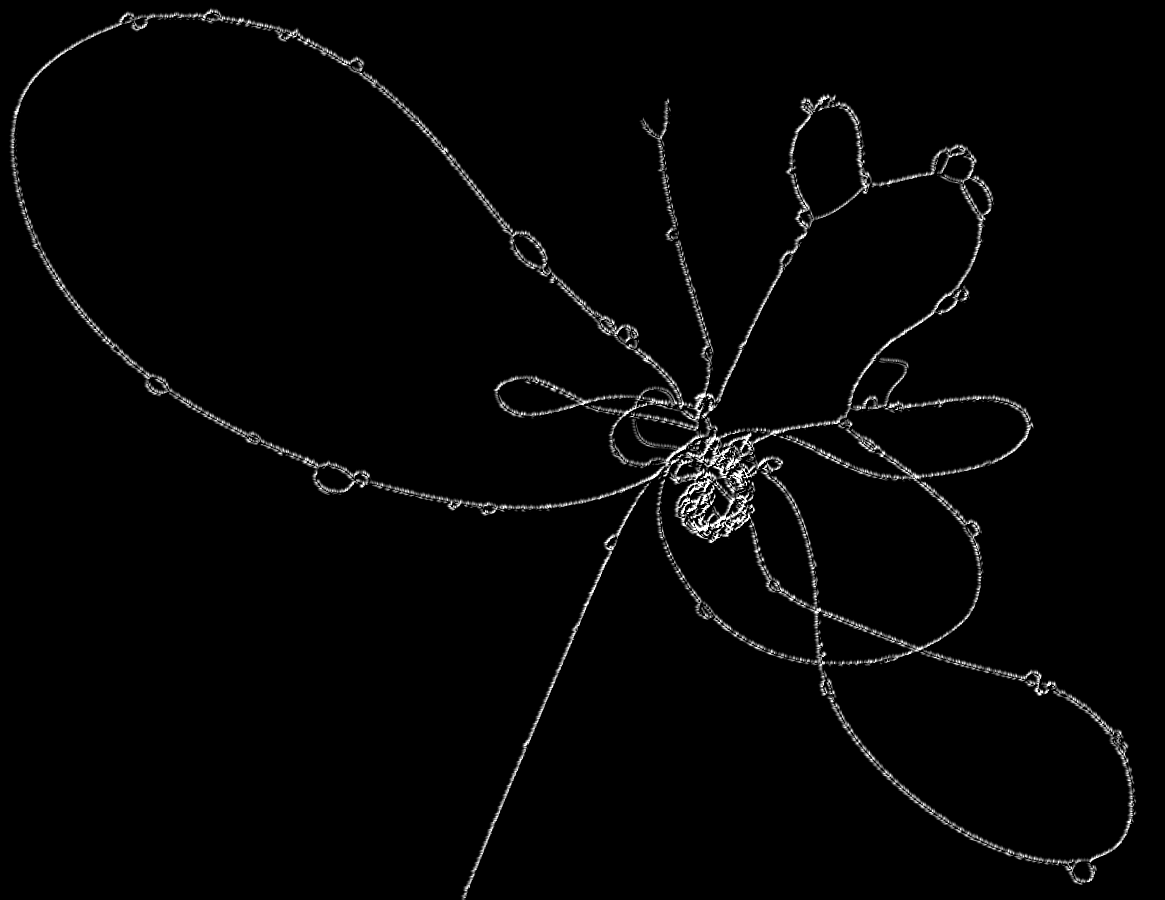
\includegraphics[width=1.0\textwidth]{figures/DRB1-3123}
\caption{\label{fig:DRB1-3123}
  A rendering of a portion of the MHC graph assembled by {\tt vg msga} around the DRB1-3123 gene.
  Node labels have been omitted. The graph rendering required enhancement to make the structure clear at this zoom level, which results in the embossed effect.
}
\end{figure}

\section{Discussion and future plans}

Presently \vg provides interfaces to the basic functions required for resequencing analysis using variation graph references.
We can construct, import, visualize, assemble, examine, modify, index, and query the graph and associated indexes using tools in \vg.
We can efficiently map new sequence reads to the reference using succinct indexes of the graph and its sequence space, and finally we can describe variation between a new sample and an arbitrary reference embedded as a path in the graph.
This framework provides the basis for future improvements and experimentation.
However, the project currently has a number of weak points which we would like to improve.

For one, the variant calling method is rudimentary and focused on determining variants against single nodes in the graph, which works for detecting SNPs and small indels.
We plan to implement a calling and genotyping approach based on superbubbles in the graph.
To do this we can employ recent work which develops a linear-time algorithm for the detection of superbubbles in the graph \cite{brankovic2016linear}.
After detecting superbubbles, we plan to apply haplotype-based variant calling approaches \cite{garrison2012haplotype} to the reads overlapping the superbubble.
This approach will be generic and handle all classes of variation, both small (SNPs and indels) and large (SVs).

Furthermore, we would like to utilize recent work generalizing the PBWT to graphs in the genotyping process.
This generalized system, gPBWT, provides the same efficient haplotype matching and counting queries possible in PBWT, but on a variation graph.
It should also be possible to apply this to reduce the complexity of the indexing process by generating a deBruijn graph for \gcsa that only contains kmers we have observed previously.
In anticipation of this, we have attempted a modification of the indexing process that only indexes the embedded paths in the graph, but have not completely debugged and tested it.

We would like to complete several experiments to validate the performance of the method in and end-to-end alignment and variant calling process.
First, we plan to complete a whole genome analysis of NA12878 and other individuals in the platinum genomes pedigree.
This is currently not possible as the calling method is localized to small regions of the graph, and we have not developed efficient techniques to extract reads overlapping a particular region.
Similarly, we plan to use sequencing data from the \href{http://www.ncbi.nlm.nih.gov/assembly/706168/}{CHM1 and CHM13} cell lines to construct a synthetic pseudodiploid.
The high quality of the \emph{de novo} assemblies for these cell lines (which are based on deep PacBio long-read sequencing) will allow us to evaluate the variation calling processes in a completely generic way within the graph itself.
We will use the calling process to generate a sample graph based on short reads and the 1000GP reference, then evaluate our results by threading the assembled contigs for CHM1 and CHM13 through the graph and counting the path divergences between them and our estimated sample graph.

In standard practice, we ignore the haplotype information in the VCF file and build the graph so as to allow all possible recombinations between successive variant loci.
This haplotype-agnostic approach has advantages of simplicity and ubiquity.
Even data providers with closed access policies often release information about the variants discovered in their cohorts, which provides a valuable resource when examining new individuals even if we do not have the complete haplotype information of the source genomes \cite{exac2015}.
However, there are valuable uses for the haplotypes, and storing this haplotype information efficiently is an area of active work among other collaborators on \vg are exploring generalizations of the positional Burrows Wheeler Transform (PBWT) \cite{durbin2014}.\footnote{Adam Novak, a collaborator on the \vg project, has implemented a generalization of the PBWT to graphs in xg. This generalization (gPBWT) is designed for efficient haplotype matching and frequency queries, but does not provide efficient positional queries.}

A large number of organisms lack complete reference genomes, or have such high rates of heterozygosity that generating linear versions of their genomes may be practically impossible.
We plan to apply \vg to these contexts by generating assembly graphs with other methods and then using these graphs as a reference for resequencing analysis.
This would allow whole genome resequencing analysis in previously-inaccessible contexts, such as in pooled sequencing of organisms without the aid of a finished reference sequence. 
Validating these approaches will require the extension of methods for population structure and association analysis to the graph, which will be a difficult but essential step in the generalization of genomics from linear to graphical systems.

\bibliography{references}{}

\bibliographystyle{plain}

\appendix


We implement efficient local alignment to variation graphs by developing a SIMD-accelerated\footnote{Single input multiple data (SIMD) instructions allow vectorized mathematical operations in a single machine instruction, and can be used to greatly speed up algorithms which may be implemented in terms of operations on vectors.} string to graph alignment algorithm. We then enable alignment against completely generic graphs by a transformation process that projects a cyclic and bidirectional graph into an acyclic, unidirectional (single-stranded) graph which preserves the sequence space of the original graph up to a given length.

\subsubsection{Background}


As our sequence graphs are models of regular languages, they can be considered equivalent to regular expressions, so we understand this result to hold for variation graphs as well.
By transforming our graph from a cyclic to acyclic format, we produce a performant implementation of the limited case of alignment between strings and regular languages. However, we have not implemented the general case of alignment between regular languages, and know of no available software methods that implement it.

\subsubsection{SIMD-accelerated local alignment}

We implement a 
We interface with GSSW by \href{https://github.com/vgteam/vg/blob/fbcb6e62/src/vg.cpp#L6461-L6532}{transforming our graph into the internal graph used by GSSW}.
This graph is acyclic and only represents a single strand of the DNA.
In order to align against completely general, bidirectional sequence graphs (such as those with cycles and inversions), we can apply several transformations to the graph first to generate a DAG with the property that we can find any sequence up to a given length $k$ from our source graph in it.

These two operations are $unfold$, which expands the graph to include its reverse complement where accessible via an inversion, and $kDAGify$, which unrolls strongly connected components of the graph ``far enough'' that we are guaranteed to be able to find any sequence of length $k$ in the source graph in the unrolled one.
This allows us to align any sequence of up to length $k$ against a completely general variation graph.
Through these steps we retain a mapping from old node ids to new ones, which we will use to project alignments to the transformed graph back into our base coordinate space.

\subsubsection{Unfolding}

In \href{https://github.com/vgteam/vg/blob/fbcb6e62/src/vg.cpp#L8289-L8400}{{\tt VG::unfold}} we use a breadth first search starting at every inverting edge in the graph to explore the reverse complemented portions of the graph that we reach in some length $k$ from the inverting edge.
We then copy this subgraph, take its reverse complement, and replace the inverting edges connecting it to the forward strand of the graph with non-inverting ones.
If $k$ is greater than any length in our graph, then we will duplicate the entire reverse complement of the graph on the forward strand, effectively doubling the size of the graph if we have any inversions in it, as shown in figure \ref{fig:unfold}.

\begin{figure}[t]
\centering
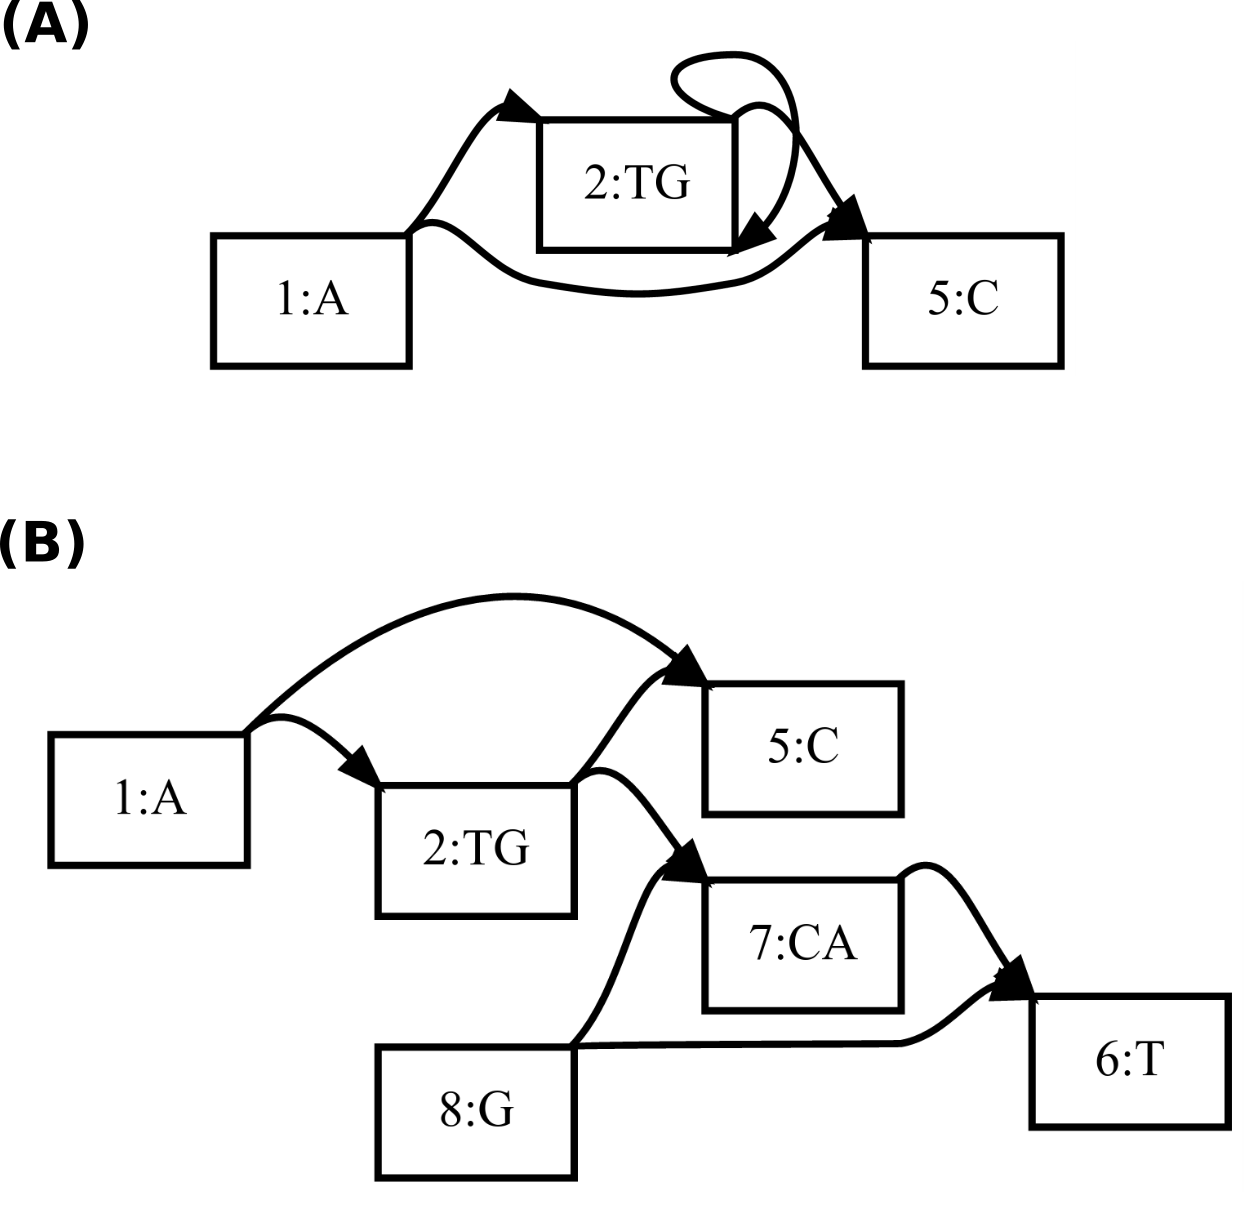
\includegraphics[width=1.0\textwidth]{figures/unfold}
\caption{\label{fig:unfold}
  Illustration of the unfolding process. The starting graph (A) has an inverting edge leading from the forward to reverse strand of node 2.
  In (B) we unroll the graph with $k$ greater than the length of the graph, which materializes the implied reverse strand as sequence on the forward strand of new nodes.
}
\end{figure}

\subsubsection{kDAG-ification}

Variation graphs may have cycles.
These are useful as compact representations of copy number variable regions, and arise naturally in the process of genome assembly.
However, partial order alignment cannot handle these structures, and so we must convert them into an approximately equivalent acyclic graph in order to align with GSSW.
To do so, we unroll cyclic structures by copying their internal nodes an appropriate number of times to allow a given query length to align through the unrolled version of the component.

We first detect all strongly connected components by using a \href{https://github.com/vgteam/vg/blob/fbcb6e62/src/vg.cpp#L3508-L3552}{recursion-free implementation} of Tarjan's strongly connected components algorithm \cite{tarjan1972depth}.
Then, we copy each strongly connected component and its internal edges into a new graph.
We greedily break edges in this graph that introduce cycles.
Now, we k-DAGify the component progressively copying the base component and for each edge between nodes in the component, connecting from the source node in the previous copy to the target node in the current copy.

We use dynamic programming to track the minimum distance back through the graph to a root node outside the component at each step.
When this reaches our target $k$, we stop unrolling, and add the expanded component back into the graph by reconnecting it with its original neighborhood.
For each copy of a node in the DAG-ified component we copy all of its inbound and outbound edges where the other end of the edge lies outside the strongly connected component.
The resulting graph is acyclic and supports queries up to length $k$ on the original graph provided the translation between the new graph and the source one.
Figure \ref{fig:kdagify} provides a visual description of the process.

\begin{figure}[t]
\centering
\includegraphics[width=1.0\textwidth]{figures/kdagify}
\caption{\label{fig:kdagify}
  Illustration of the unrolling process. The starting graph (A) and a representation without sequences or sides to clarify the underlying structure (B).
  In (C) we have unrolled one step ($k = 2$). In (D), $k = 4$, (E) $k = 10$, and (F) $k = 25$.
}
\end{figure}

\subsection{Succinct graph representation ({\tt xg})}

When using a variation graph as a reference system, we are unlikely to need to modify it.
As such we can compress it into a system that provides efficient access to important aspects of the graph.
Specifically, we care about the node and edge structure of the graph and queries that allow us to extract and seek to positions in embedded paths.
We would like to be able to query a part of the graph corresponding to a particular region of a chromosome in a reference path embedded in the graph.
Similarly, if we find an exact match on the graph using \gcsa, we would like to load that region of the graph into memory for efficient local alignment.

We implement a succinct representation of the graph in the \href{https://github.com/vgteam/xg}{{\tt xg}} library.
We do so using data structures from \href{https://github.com/simongog/sdsl-lite}{SDSL-lite}, which provides \href{https://en.wikipedia.org/wiki/Succinct_data_structure#Succinct_dictionaries}{rank/select dictionaries} that we use to navigate compressed vectors that record the labels and id space of the nodes, edges, and paths of the graph \cite{okanohara2007}.
Our model is summarized visually in figure \ref{fig:xg}.

\subsubsection{Storing the nodes of the graph}

We first concatenate node labels to generate the node sequence vector $V_s = seq(n_1) + seq(n_2) + \ldots + seq(n_{|N|})$.
We store this as a compressed integer vector using the minimum required number of bits per base (which is typically 3 bits, as we need to represent ${\tt A, T, G, C, N} \}$).
In a second bit vector $V_b : |V_b| = |V_s|$ (the node bit vector), we write 1 at the position corresponding to the first base in every node in $V_s$, and write a 0 for all internal bases.
We then store the node ids in the wavelet tree $V_i$ \cite{grossi2003high}, ordered by their appearance in $V_s$.

By building a rank/select dictionary from $V_b$, we can map from positions in the sequence vector to node ids, and from node ids to ranges in the sequence vector.
For example, we can look up the sequence of a particular node by its id in several steps.
We first query the node id wavelet tree to obtain the rank $n$ of a particular node by its id $i$: $n = rank_{i}(V_i, 1)$.
Then, $select_1(V_b, n)$ will return the position of the start of the $n$th node in the node sequence vector.
In reverse, we can use $rank_1(V_s, n)$ to map from positions in $V_s$ to node ranks, and then find the node id as $V_i[n]$.
Recording the node identifiers in $V_i$ allows us to work with non-contiguous node id spaces, but internally within {\tt xg}, we identify nodes by their rank in $V_s$ and $V_i$.

\subsubsection{A succinct bidirectional encoding of the edges of the graph}

Variation graphs which we are likely to use as a reference system tend to have few nodes with a high in or out degree.
We rely on this tendency to generate a bidirectional index of edges that is optimized for sparsely-connected graphs.

We store the edges of graph, $E$, using a pair of compressed integer vectors $F_e$ and $T_e$.
In each vector, we record information about the edges of each node in a single range of the vector.
We record the ranges of these vectors corresponding to particular nodes by marking bit vectors $F_b$ and $T_b$.

We record the edges in the forward direction in $F_e$.
For each $n_i \in N$ we write its own id into $F_e$.
Then for each edge from that node ($\forall j : e_{n_i \rightarrow j}$) we record the id of the node it goes to ($j$) in a block after the entry for $n_i$.
We record the position of the node blocks in $F_e$ in $F_b$ by marking the node entry with a 1, and leaving edge entries as 0.

$T_e$ and $T_b$ follow the same pattern, but instead of recording the edges from a node, we record the edges to it.
This bidirectional structure allows for fast traversal of the graph.
Note that $|F_e| = |T_e| = |N| + |E|$.
In other words, these vectors encode one entry for each node and edge in the graph.
We can exploit this property to provide a unique rank-based identifier for every node and edge in the entity space of the graph, which is useful for marking subgraphs with particular properties.

We use such a pattern to record the which node strand each edge starts and ends on.
Four additional bit vectors mark whether an edge starts or ends on the forward or reverse strand: $|I_f| = |I_t| = |J_f| = |J_t| = |N| + |E|$.
We first mark all positions corresponding to the node block starts in $F_e$ as 0.
This padding ensures that we are working in the graph's entity space as described by $F_e$.
In $I_f$ we record if an edge in $F_e$ begins on the reverse strand (1) or not (0), and in $J_f$ we do the some for edges as described in $T_e$.
In $I_t$ we store if an edge in $F_e$ goes to the reverse strand (1) or not (0), while $J_t$ lets us do the some for edges as ordered in $T_e$.
In directed graphs these are typically sparse and easily compressible, but they are necessary to represent completely generic graphs.

\subsubsection{Compact path storage allowing positional queries}

In {\tt xg} we develop a compact representation of embedded paths that allows them to be used for $O(1)$ time positional queries.
For each path $p_j$ we store a bit vector $C_p^j$ with the same length as our forward edge vector $F_e$.
We mark 1 in this vector for each element in the graph which occurs in the path at its corresponding position in $F_e$, and a 0 otherwise.

We record the positions of the mappings ($m_1, \ldots, m_{|p_j|}$) of $p_j$ in an integer vector $M_p^j$, where we record the node ranks of the nodes the path traverses in $V_s$.
The strand of each mapping $m$ is marked in a bit vector $S_p^j$ of the same length as $M_p^j$.
We mark 0 if the mapping traverses the node's forward strand and 1 if it traverses the reverse.

Finally, we build a positional index of the path that allows us to determine what node strand of the path is at a given position.
We cache the start position of each node relative to the beginning of the path in $L_p^j : |L_p^j| = |M_p^j|$.
The bit vector $B_p^j$ has the same length as the sequence represented by the path.
For each position in the path where we begin a node, we mark a 1, and leave 0 otherwise.
We can now determine the node at a given position $x$ in the path as $M_p^j[rank_1(B_p^j, x)]$.
Furthermore, we can efficiently determine where in a particular path a node is using the $L_p^j$ vector.
This representation is not lightweight, and does not allow the storage of many paths because it requires $O(\sum_{\forall p \in P}{|p|})$ space.
However, it is an essential component of the index if we wish to query the graph based on the coordinate system of an existing linear reference sequence.

\begin{figure}[t]
\centering
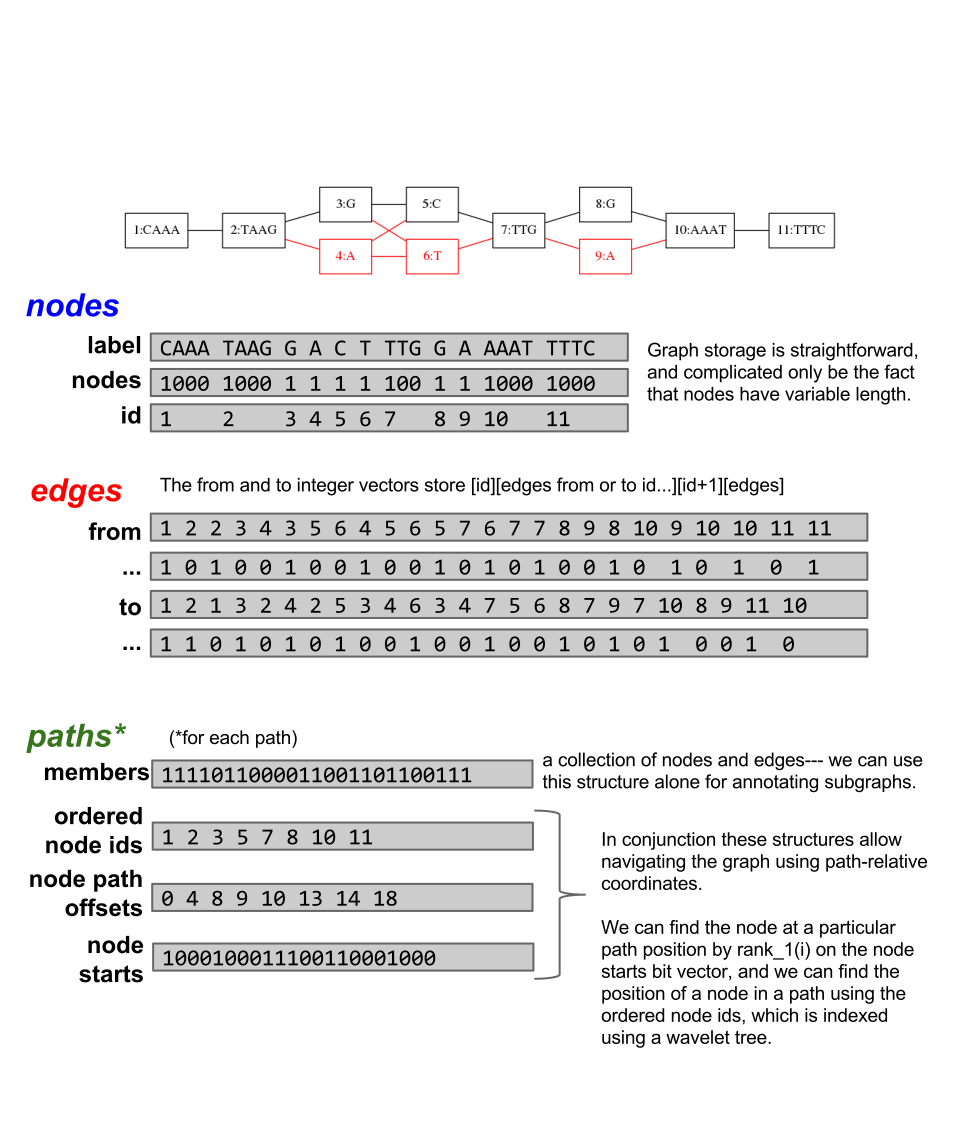
\includegraphics[width=1.0\textwidth]{figures/xg}
\caption{\label{fig:xg}
  A sketch of important components of the {\tt xg} graph index.
  The source graph is at the top of the figure.
  A single path is defined by the nodes and edges in black.
  For simplicity we omit the edge type vectors and the traversal orientation vector as in this directed acyclic graph they would be marked as 0.
}
\end{figure}

\section{Implementation}

Dependencies on \href{}{xg}, \href{}{GCSA2}, and various libraries including \href{}{SDSL}. 
Protobuf for serialisation onto disk.

\subsection{Software development and continuous integration testing}

All features of \vg are validated after every update to the source repository using \href{https://travis-ci.org/vgteam/vg}{continuous integration software validation approaches}.
As such, basic tests demonstrate the desired functionality for each feature, in some cases in using a programmatic proof.
For example, we use kmer matching to verify that the kmer space of a graph is equivalent before and after unrolling and kDAGification.
As of this writing, we have implemented 228 tests validating the functionality of the system.


\end{document}
